\documentclass[a4paper,12pt]{article}
\usepackage[margin=0.75in]{geometry}
\usepackage[utf8]{inputenc}
\usepackage{exsheets}

\DeclareInstance{exsheets-heading}{block-no-nr}{default}{
	attach = {
		main[l,vc]title[l,vc](0pt,0pt) ;
		main[r,vc]points[l,vc](\marginparsep,0pt)
	}
}
\RenewQuSolPair
{question}[headings=runin]
{solution}[headings=block-no-nr]

\SetupExSheets{
	counter-format=qu.,
	solution/print=true ,
	question/name=Feladat,
	solution/name=Megoldás.
}

\SetupExSheets{solution/print=true}
\SetupExSheets{question/name=}
\SetupExSheets{headings=runin}

\usepackage[hungarian]{babel}
\usepackage{amsmath}
\usepackage{mathtools}
\usepackage{amsthm}
\usepackage{amsfonts}
\usepackage{amssymb}
\usepackage{graphicx}
\graphicspath{{./images/}}
\usepackage{stuki}
\usepackage{stukicommands}
\usepackage{float}
\usepackage{wrapfig}
\usepackage{minted}

\usepackage{titling}
\setlength{\droptitle}{-2cm}

\theoremstyle{definition}
\newtheorem{definition}{Definíció}
\newtheorem*{definition*}{Definíció}
\newtheorem*{remark}{Megjegyzés}
\newtheorem{theorem}{Tétel}
\newtheorem*{theorem*}{Tétel}

\title{\huge{Algoritmusok és adatszerkezetek II} \\[-4pt] \large \vspace{-15pt}}
\author{Boda Bálint}
\date{\vspace{-12pt}2022. őszi félév}

\usepackage{animate}

\begin{document}
	\maketitle
	\section{Minimális feszítőfák(MST)}
	\subsection{Kruskal algoritmus}
	\begin{tasks}
		\task{
			A Kruskal algoritmus egy tetszőleges $G$ gráf egy minimális feszítőerdejét állítja elő. Az algoritmus továbbá visszaad egy számot ami, ha 1 a gráf összefüggő. Nyilván ekkor a feszítőerdő egyetlen egy komponensből áll, azaz egy feszítőfa.
		}
	
		\task{
			\begin{figure}[H]
				\begin{center}
					\animategraphics[controls, scale=0.75]{1}{kruskal}{0}{7}
				\end{center}
			\end{figure}
		}
	
		\task{
			\begin{theorem*}
				Ha a $ G = (V, E) $ irányítatlan, összefüggő, élsúlyozott gráfon
				\begin{enumerate}
					\item az $A$ élhalmaz részhalmaza $G$ valamelyik minimális feszítőfája élhalmazának
					\item az $ (S, V \setminus S) $ vágás elkerüli az $A$ élhalmazt
					\item $(u,v) \in E$ könnyű él az $(S, V \setminus S)$ vágásban,
				\end{enumerate}
				akkor az $(u,v)$ él biztonságosan hozzávehető az $A$ élhalmazhoz.
			\end{theorem*}
			\vspace{8pt}
			\begin{definition*}
				A $G = (V, E)$ irányítatlan összefüggő gráf feszítőfája a $T = (V,F)$ gráf, ha $F \subseteq E$ és $T$ fa.
			\end{definition*}
			\vspace{8pt}
			\begin{definition*}
				A $G$ irányítatlan összefüggő élsúlyozott gráf \textbf{minimális feszítőfája} (angolul: minimum spanning tree) $T$, ha $T$ feszítőfája $G$-nek és $G$ bármely $T'$ feszítőfája esetén:
				\[
				w(T) \le W(T')
				\]
			\end{definition*}
			\vspace{8pt}
			\begin{definition*}
				Legyen $G = (V,E)$ egy gráf. Ha $ \emptyset \ne S \subset V $, akkor az $(S,V \setminus S)$ gráfot vágásnak nevezzük.
			\end{definition*}
			\vspace{8pt}
			\begin{definition*}
				A $G = (V,E)$ gráf, egy $(u,v)$ éle keresztezi a $(S,V \setminus S)$ vágást, ha
				\[
				(u \in S \land v \in V \setminus S) \lor (u \in V \setminus S \land v \in S)
				\]
			\end{definition*}
			\vspace{8pt}
			\begin{definition*}
				A $G = (V,E)$ gráfban az $(S,V \setminus S)$ vágás elkerüli az $A \subseteq E$ élhalmazt, ha $A$ egyetlen éle sem keresztezi a vágást. 
			\end{definition*}
			\vspace{8pt}
			\begin{definition*}
				A $G = (V,E)$ élsúlyozott gráf egy $(u,v) \in E$ élét könnyű élnek nevezzük, ha keresztezi az $(S,V \setminus S)$ vágást, és költsége kisebb vagy egyenlő mint bármely más a vágást keresztező élé.
			\end{definition*}
			\vspace{8pt}
			\begin{definition*}
				Tegyük fel, hogy $G = (V,E)$ élsúlyozott, irányítatlan, összefüggő gráf és $A$ részhalmaza $G$ valamely minimális feszítőfája élhalmazának. Ekkor az $(u,v) \in E$ él biztonságosan hozzávehető az $A$ élhalmazhoz, ha $(u,v) \notin A$ és $A \cup \{(u,v)\} $ részhalmaza $G$ valamely minimális feszítőfája élhalmazának.
			\end{definition*}
		}
		\task{
			A Kruskal algoritmus invariánsa miatt teljesülnek a tétel feltételei, ezáltal egy adott él az algoritmus futása során, $A$-hoz csak biztonságos éleket veszünk.
		}
		\task{
			\begin{figure}[H]
				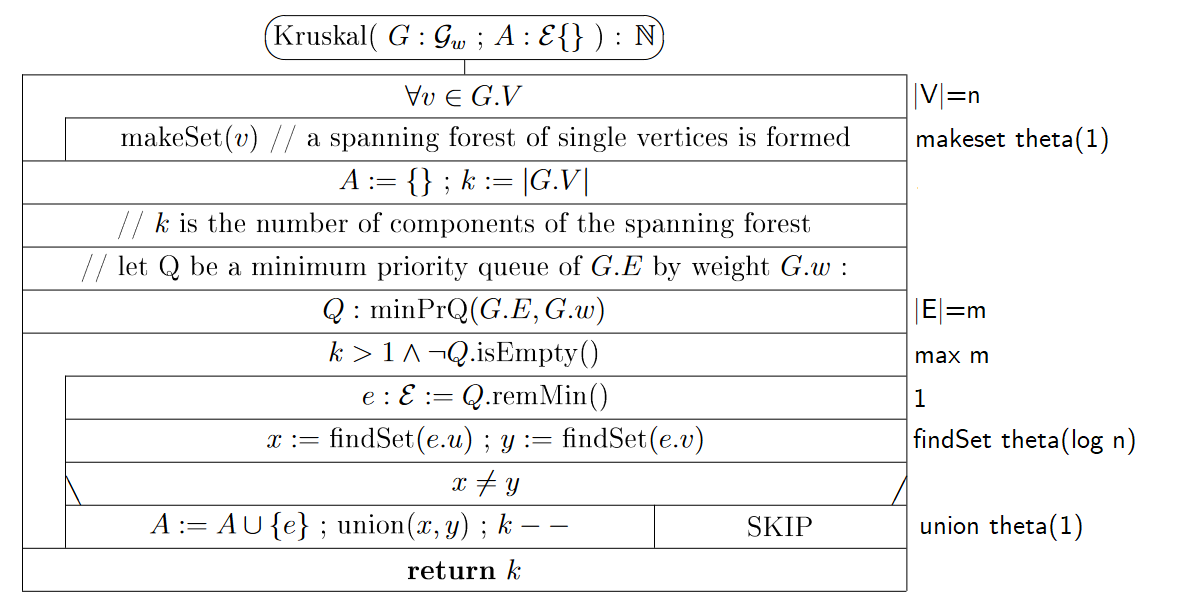
\includegraphics[scale=0.5]{kruskalmuv}
			\end{figure}
			Így a műveletigény: $(n + m + m \cdot \log n) \in \Theta(m \cdot \log n)$, ha feltesszük, hogy a \mintinline{pascal}|makeSet| és \mintinline{pascal}|union| műveletek műveletigénye $ \Theta(1) $ a \mintinline{pascal}|findSet|-é pedig $ \Theta(\log n) $, illetve a minimum prioritásos sor inicializálása $ \Theta(m) $, a \mintinline{pascal}|remMin()| metódus költsége pedig max. $ \Theta(\log m) $.
		}
	\end{tasks}
	\newpage
	\subsection{Prim algoritmus}
	\begin{tasks}
	\task{A Prim algoritmus egy összefüggő élsúlyozott irányítatlan gráf egy minimális feszítőfáját adja meg.}
	\task{
		\begin{figure}[H]
			\begin{center}
				\animategraphics[controls, scale=0.75]{1}{prim1-}{0}{8}
			\end{center}
		\end{figure}
	}
	\task{
		\begin{theorem*}
			Ha a $ G = (V, E) $ irányítatlan, összefüggő, élsúlyozott gráfon
			\begin{enumerate}
				\item az $A$ élhalmaz részhalmaza $G$ valamelyik minimális feszítőfája élhalmazának
				\item az $ (S, V \setminus S) $ vágás elkerüli az $A$ élhalmazt
				\item $(u,v) \in E$ könnyű él az $(S, V \setminus S)$ vágásban,
			\end{enumerate}
			akkor az $(u,v)$ él biztonságosan hozzávehető az $A$ élhalmazhoz.
		\end{theorem*}
		\vspace{8pt}
		\begin{definition*}
			A $G = (V,E)$ élsúlyozott gráf egy $(u,v) \in E$ élét könnyű élnek nevezzük, ha keresztezi az $(S,V \setminus S)$ vágást, és költsége kisebb vagy egyenlő mint bármely más a vágást keresztező élé.
		\end{definition*}
		\vspace{8pt}
		\begin{definition*}
			Legyen $G = (V,E)$ egy gráf. Ha $ \emptyset \ne S \subset V $, akkor az $(S,V \setminus S)$ gráfot vágásnak nevezzük.
		\end{definition*}
	}
	\task{
		Az algoritmus egy tetszőleges csúcsból indulva elkezdi építeni a $ (V,F) $ minimális feszítőfát a $ T = (N,A) $ kezdetben egyetlen egy csúcsból álló fából. Minden lépésben $T$-hez egy újabb biztonságos élt és az ahhoz tartozó csúcsot adjuk. Így az algoritmus futása során végig igaz marad az $N  \subseteq V \land A \subseteq F $ invariáns. Ehhez minden lépésben egy könnyű élt választunk ki az $(N, V \setminus N)$ vágásban, ami a tétel miatt biztonságos él.
	}
	\task{
		\begin{figure}[H]
			\centering
			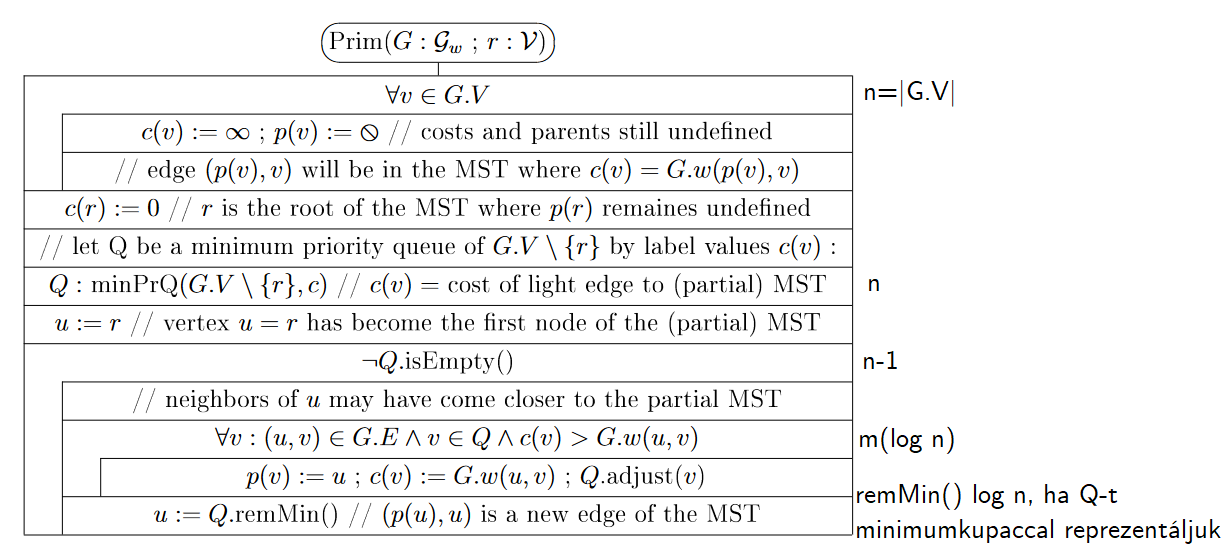
\includegraphics[scale=0.5]{prim}
		\end{figure}
		\[
		MT_{prim} \in \underbrace{\Theta(n)}_{\text{inicializáló ciklus}} + \underbrace{\Theta(n)}_{\text{minPrQ inicializálása}} + \underbrace{O(n \cdot \log n)}_{\text{külső ciklus}} + \underbrace{O(m \cdot \log n)}_{\text{belső ciklus}} \in O((n+m) \cdot log n)
		\]
	}
	\end{tasks}
	\newpage
	\section{Legrövidebb utak}
	\subsection{Dijkstra algoritmus}
	\begin{tasks}
		\task{
			Egy élsúlyozott $G$ gráf tetszőleges $s$ csúcsából optimális utat ad meg $G$ minden $s$-ből elérhető csúcsára. Minden élnek pozitív élsúlyúnak kell lennie.
		}
		\task{
		}
		\task{
			\begin{figure}[H]
				\centering
				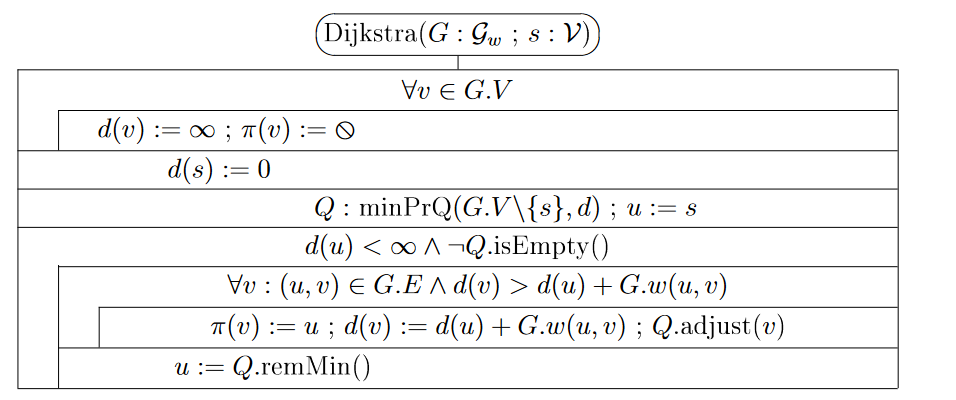
\includegraphics[scale=0.6]{dijkstra}
			\end{figure}
		}
		\task{
			Ha a prioritásos sort minimum kupacként ábrázoljuk. Ekkor az a kupac inicializálása $\Theta(n)$, az \mintinline{pascal}|adjust()| $\in \Theta(\log n) $
		}
		\task{}
		\task{
			Ekkor a \mintinline{pascal}|remMin()| eljárás műveletigénye $\Theta(n)$. Ez az eljárás a fő ciklus minden iterációjában lefut, figyelembe véve még a belső ciklust is $ MT_{Dijkstra} \in O((n+m) \cdot n)$ műveletigény adódik. A minimális esetben egyetlen egyszer fut le a külső és egyszer sem a belső ciklus így abban az esetben az minimum prioritásos sor és a $d$ és $\pi$ tömbök inicializálása lesz meghatározó, ami $ mT_{Dijkstra} \in \Theta(n) $ műveletigényt eredményez.
		}
	\end{tasks}
	\subsection{DAG legrövidebb utak algoritmus}
	\subsection{Soralapú Bellman-Ford algoritmus}
	\newpage
	\section{Mintaillesztés}
	\subsection{Brute-force}
		Nem túl hatékony:
			\begin{align*}
				mT_{BF} &\in \Theta(n) \\
				MT_{BF} &\in \Theta(n \cdot m), \text{ ami kellően nagy } m \text{ esetén } \Theta(n^2)
			\end{align*}
		ahol $n$ a szöveg $m$ pedig a minta hossza.
	\subsection{Quicksearch}
	\begin{tasks}
		\task{
			A Quicksearch algoritmus, egy $T/1: \Sigma[n]$ szövegben a $P/1: \Sigma[m]$ minta összes érvényes eltolását, azaz az
			\[
			\bigl\{ s \in [0..(n-m)] \mid T[s+1..s+n] = P[1..m] \bigr\}
			\]
			halmazt adja meg. ($[0..(n-m)]$ intervallumot míg $T[s+1..s+n]$ réssztringet jelöl)
		}
		\task{
			\begin{figure}[H]
				\begin{center}
					\animategraphics[controls]{1}{qs1-}{0}{8}
				\end{center}
			\end{figure}
		}
		\task{
			\begin{figure}[H]
				\begin{center}
					\animategraphics[controls, scale=0.75]{1}{qs2-}{0}{5}
				\end{center}
			\end{figure}
		}
		\task{
			\begin{figure}[H]
				\centering
				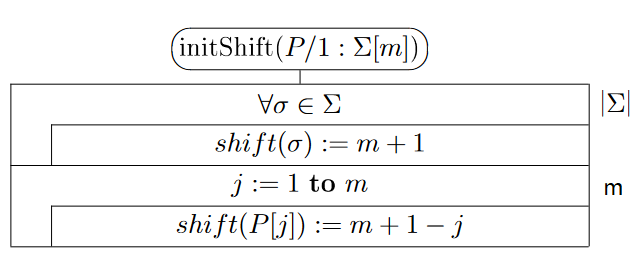
\includegraphics[scale=0.6]{qs_init_muv}
			\end{figure}
			\begin{figure}[H]
				\centering
				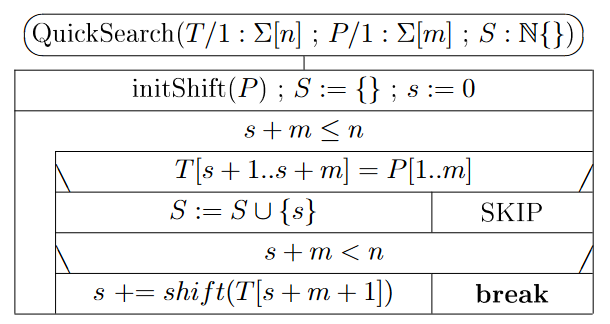
\includegraphics[scale=0.6]{qs_muv}
			\end{figure}
		}
		\task{
			\begin{align*}
				mT(n,m) &\in \Theta\left(\frac{n}{m+1} + m \right) \quad (\text{pl. ha } T[1..n] \text{ és } P[1..m] \text{ diszjunktak}) \\
				MT(n,m) &\in \Theta \bigl( (n-m+2) \cdot m \bigr) \quad (\text{pl. ha } T = AA...A \text{ és } P = A...A )
			\end{align*}
			\begin{definition*}
				Legyen $G = (V,E)$ egy gráf. Ha $ \emptyset \ne S \subset V $, akkor az $(S,V \setminus S)$ gráfot vágásnak nevezzük.
			\end{definition*}
		}
		\task{
			Maximális futási ideje rosszabb mint a többi algoritmusnak. Átlagos futási ideje rosszabb mint a KMP algoritmusnak és a visszalépések miatt nem használható szekvenciális fájlokon egy ideiglenes tárhely bevezetése nélkül.
		}
	\end{tasks}
	\newpage
	\subsection{KMP}
	\begin{tasks}
		\task{
			A KMP algoritmus, egy $T/1: \Sigma[n]$ szövegben a $P/1: \Sigma[m]$ minta összes érvényes eltolását, azaz az
			\[
			\bigl\{ s \in [0..(n-m)] \mid T[s+1..s+n] = P[1..m] \bigr\}
			\]
			halmazt adja meg. ($[0..(n-m)]$ intervallumot míg $T[s+1..s+n]$ réssztringet jelöl)
		}
		\task{
			\begin{figure}[H]
				\begin{center}
					\animategraphics[controls]{1}{init1-}{0}{10}
				\end{center}
			\end{figure}
			Így a $next$ tömb a következő: \\
			\begin{tabular}{c|c|c|c|c|c|c|c|c}
				$P[j]$ & B & A & B & A & A & B & A & B \\
				\hline
				$j$ & 1 & 2 & 3 & 4 & 5 & 6 & 7 & 8 \\
				\hline
				$next[j]$ & 0 & 0 & 1 & 2 & 0 & 1 & 2 & 3 \\
			\end{tabular}
		}
		\task{
			\begin{figure}[H]
				\begin{center}
					\animategraphics[controls, scale=0.75]{1}{kmp1-}{0}{31}
				\end{center}
			\end{figure}
			Így $S = \{3,8,15\} $.
		}
		\task{
			\begin{figure}[H]
				\centering
				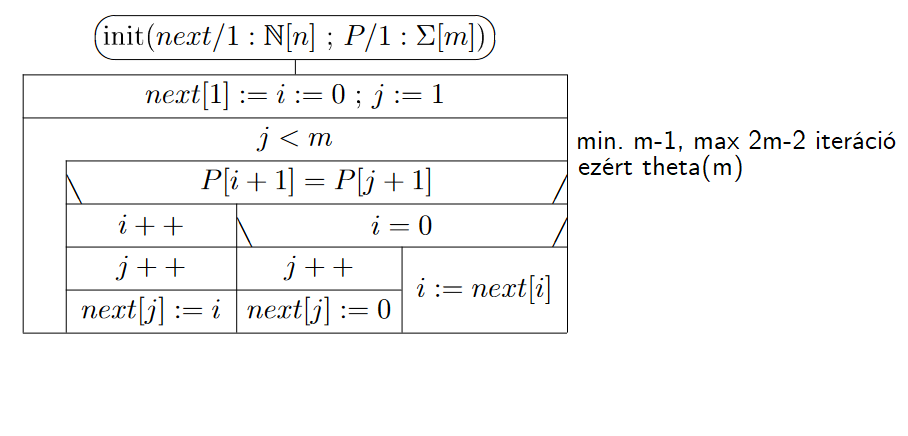
\includegraphics[scale=0.5]{kmp_init_muv}
				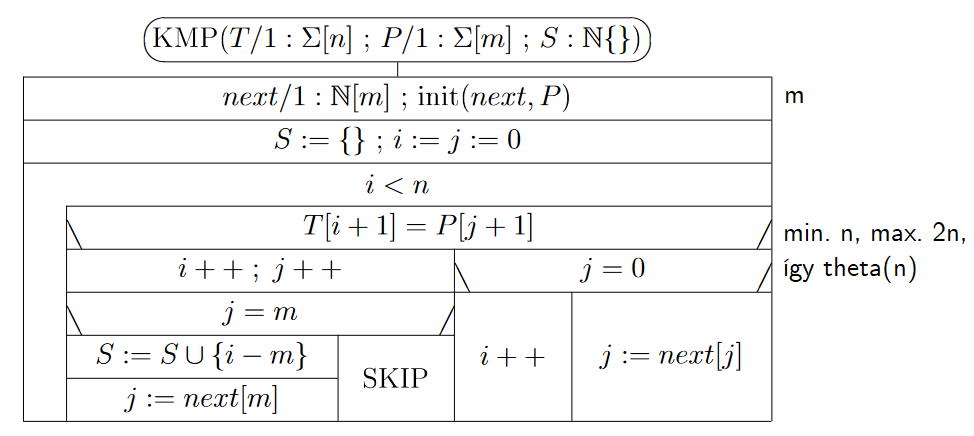
\includegraphics[scale=0.5]{kmp_muv}
			\end{figure}
		}
		\task{
			Az \mintinline{pascal}|init()| függvény ciklusa minimum $m-1$, maximum $2m-2$ alkalommal iterál így műveletigénye $\Theta(m)$. A fő eljárás ciklusa legalább $n$-szer, legfeljebb $2n$-szer iterál, továbbá egyszer lefut az inicializáló függvény, így $m_{KMP} \in \Theta(m + n) = \Theta(n) $.
		}
		\task{
			A KMP algoritmus műveletigénye jobb, továbbá, mivel az algoritmus során nem lépünk vissza a $T$ szövegben, ezért szekvenciális inputfájlokkal is használható átmeneti tároló bevezetése nélkül.
		}
	\end{tasks}
\end{document}